% !TeX root = l4saqm_tr.tex
% ================================================================
\section{Introduction}\label{l4saqmtr_intro}

The DualQ Coupled AQM~\cite{DeSchepper15b:DCttH_TR, Briscoe15e:DualQ-Coupled-AQM_ID} was proposed as a way to provide a Low Latency Low Loss and Scalable throughput (L4S) service that would be usable for all Internet traffic, while doing no harm to existing non-L4S (`Classic') traffic. 

To preserve the low latency service, L4S traffic has to use a so-called `Scalable' congestion control. DCTCP~\cite{Alizadeh10:DCTCP} is a good example for elastic traffic, but it needs some minor safety and performance modifications for use on the public Internet; termed the `TCP Prague `requirements~\cite{Briscoe15f:ecn-l4s-id_ID}. Other scalable congestion controls are being developed, for instance for real-time applications.

\begin{figure}[h]
	\centering
	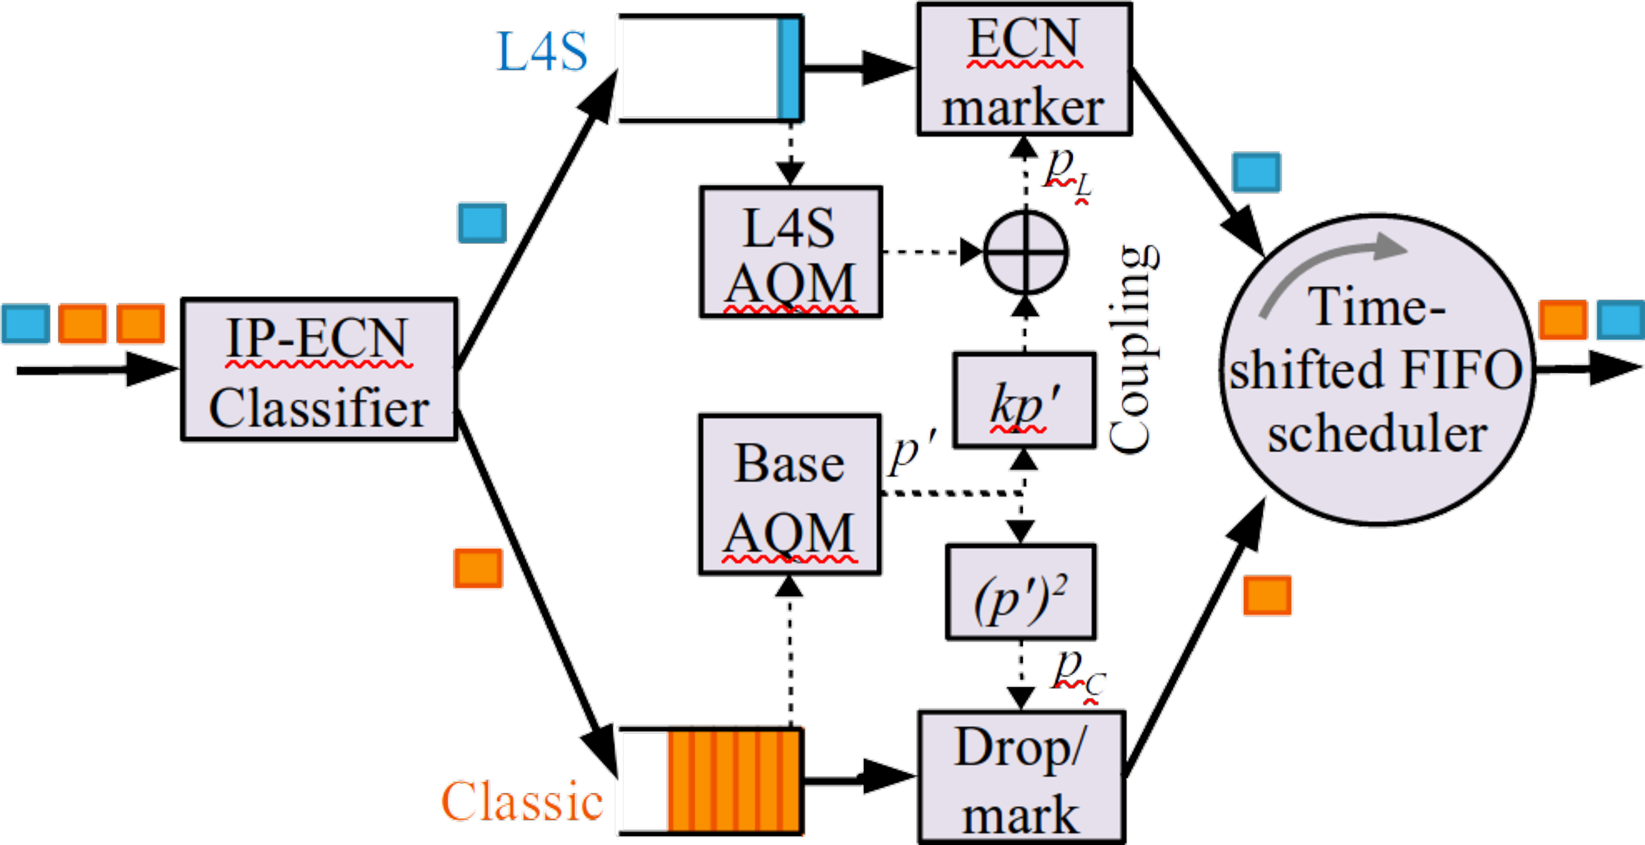
\includegraphics[width=\columnwidth]{aqm-dualq-coupled}
	\caption{DualQ Coupled AQM}\label{fig:aqm-dualq-coupled}
\end{figure}

The Dual AQM is shown in \autoref{fig:aqm-dualq-coupled} where the two queues for L4S and Classic traffic can be seen. Each queue is regulated by its own native AQM, but the AQM for Classic traffic serves as a Base AQM both for Classic traffic and for to couple the marking of L4S traffic to that of Classic. 

Coupled marking is necessary for coexistence between L4S and Classic traffic, without the former starving the latter. As shown in the figure, marking from the base AQM is applied linearly to L4S traffic, but squared before applying to Classic traffic. The squaring counterbalances the square root in the Classic TCP rate equation, so that each flow ends up using roughly the same share of the total link capacity, irrespective of whether it is a Classic or a L4S flow (see the above references for details).

The DualQ Coupled AQM includes a native L4S AQM to regulate L4S traffic on its own. When both L4S and Classic traffic are present, L4S traffic is marked if either the base AQM or the native L4S AQM decide to mark it, which is shown as a logical OR symbol (\(\oplus\)) in the figure.

When the DualQ Coupled AQM was first proposed, the L4S AQM was implemented and evaluated as a simple step ECN marking function based on the instantaneous queue length, given this was already proven for DCTCP. Nonetheless, subsequent work has highlighted some issues with this simple AQM. 

This memo focuses solely on the native L4S AQM and proposes various improvements to the original step design. One motivation for DCTCP to use simple step marking was that it was possible to deploy it by merely configuring the RED implementations in existing hardware, albeit in an unexpected configuration by setting parameters to degenerate values. However, there is no longer any imperative to stick with the original DCTCP step-function design, because changes will be needed to implement the DualQ Coupled AQM anyway, and the requirements for L4S congestion controls are not yet set in stone either.

Briefly, the solutions explored in this memo are:
\begin{itemize}
	\item Using a virtual queue
	\item Gradient marking, that is, using a (steep) ramp or convex function rather than an on-off step
\end{itemize}

An introductions to the issues that each of these solutions addresses is given at the start of each individual section about the solution. These solutions can each be applied independently or in any combination, including using all of them.

\subsection{The Current Native L4S AQM}\label{l4saqmtr_current}

The current reference software implementation of the DualQ Coupled AQM for Linux (specified as pseudocode in Appendix A of \cite{Briscoe15e:DualQ-Coupled-AQM_ID}) has already been changed from the original DCTCP-based design. This is because configuration of a step threshold in units of bytes depends on the drain rate, but the drain rate of the L4S queue continually varies depending on the proportion of Classic traffic competing for the link. Evaluations have proved that the original queue-length-based measurement led to increased L4S queuing delay when Classic traffic was present (because a certain number of bytes in a queue clearly takes longer to drain when the drain rate is reduced).

It has subsequently been proposed by others as well that the DCTCP step function ought to be configured in time units---for the similar reason that the drain rate might vary if the queue is part of a larger scheduling hierarchy~\cite{Nichols12:CoDel, Bai16:MQ-ECN, Bai16:ECN_GPS}.

Therefore, the current L4S native AQM uses the sojourn time of each packet to measure the L4S queue in units of time, not bytes. It marks a packet if the sojourn time is greater than a fixed time threshold (1\,ms for the public Internet) unless the queue length (in bytes) is less than 2 MTU. The latter condition is necessary to prevent excessive marking in cases where the drain rate is very low, so that a 1\,ms threshold would represent less than 2 full-sized packets. Otherwise the resulting marking would severely under-utilize the link.




